\documentclass[journal,article,submit,pdftex,moreauthors]{Definitions/mdpi}
\usepackage[english]{babel}
% Localización de los rótulos incluidos literalmente en la clase MDPI.
\usepackage{tikz}
\usetikzlibrary{babel}
\usetikzlibrary{arrows.meta,positioning}

\firstpage{1}
\makeatletter\setcounter{page}{\@firstpage}\makeatother
\pubvolume{1}
\issuenum{1}
\articlenumber{0}
\pubyear{2026}
\copyrightyear{2026}
\datereceived{}
\daterevised{}
\dateaccepted{}
\datepublished{}
\hreflink{}
\Title{Mismatch between field of study and employment among STEM university graduates in Ecuador: a machine learning approach}
\TitleCitation{Mismatch between field of study and employment among STEM university graduates in Ecuador}
% ORCID supplied by the authors in their previous LaTeX document.
\newcommand{\orcidauthorA}{0000-0001-5682-9705}
\newcommand{\orcidauthorB}{0009-0008-1980-6086}
\newcommand{\orcidauthorC}{0000-0002-1691-1947}
\Author{Harolt S. Farinango Palacios $^{1,*}$\orcidA{}, Steven Pa\'{u}l Rodr\'{i}guez Guerrero $^{1}$\orcidB{} and Kevin Andr\'{e}s Erazo Y\'{e}pez $^{1}$\orcidC{}}
\AuthorNames{Harolt S. Farinango Palacios, Steven Pa\'{u}l Rodr\'{i}guez Guerrero and Kevin Andr\'{e}s Erazo Y\'{e}pez}
\AuthorCitation{Farinango Palacios, H.S.; Rodr\'{i}guez Guerrero, S.P.; Erazo Y\'{e}pez, K.A.}
\address{%
$^{1}$ \quad School of Mathematical and Computational Sciences, Yachay Tech University, Hacienda San Jos\'{e} s/n, San Miguel de Urcuqu\'{i} 100119, Ecuador; harolt.farinango@yachaytech.edu.ec (H.S.F.P.); steven.rodriguez@yachaytech.edu.ec (S.P.R.G.); kevin.erazo@yachaytech.edu.ec (K.A.E.Y.)}
\corres{ harolt.farinango@yachaytech.edu.ec}
\abstract{Obtaining a university degree and entering the labour market do not guarantee a match between education and occupation. This study classifies mismatch by field of study amongst employed individuals with STEM university degrees in Ecuador, using annual ENEMDU microdata from 2021 to 2025. The research is quantitative, observational and predictive. A normative label was constructed using educational and occupational classifications and an adaptation of Montt's correspondence. Logistic regression, Random Forest and XGBoost were compared using 2021--2023 for development, 2024 for validation and 2025 for temporal testing. Of 24,895 eligible person-period records, 24,525 were evaluable. Weighted mismatch in 2025 was 40.28\% (approximate 95\% bootstrap interval: 36.70--44.63\%). The median nominal labour income was USD 898 among compatible records and USD 663 among mismatched records. Logistic regression achieved the highest ROC-AUC (0.6522), whereas XGBoost achieved the highest average precision (0.5673) and Random Forest the highest balanced accuracy (0.5931). Sex, STEM field and province were among the most important predictors. Sensitivity analyses showed modest changes in discrimination after excluding 2021 and potentially overlapping households. These findings support a descriptive assessment of observed educational and occupational matching, but predictive performance remains limited and the results do not establish causality or measure unfilled vacancies. The code and replication materials are available at \url{https://github.com/Steven735-star/Ecuador-STEM-Mismatch-2021-2025}.}
\keyword{field-of-study mismatch; STEM graduates; ENEMDU; machine learning; Ecuador}

\begin{document}
\begin{center}
\textbf{Graphical Abstract}\par\smallskip
\resizebox{\linewidth}{!}{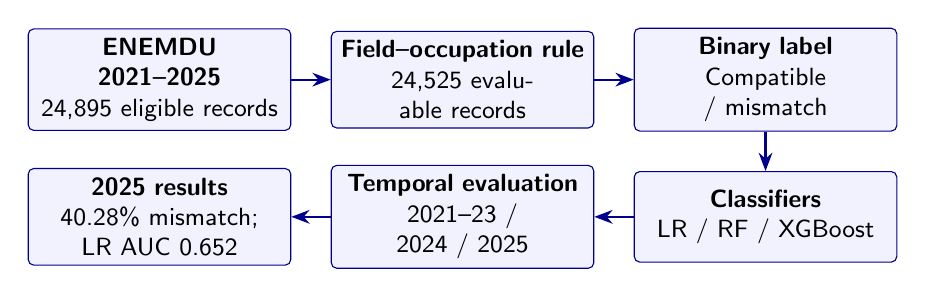
\begin{tikzpicture}[node distance=5mm, every node/.style={font=\sffamily\small}, stage/.style={draw=blue!55!black,fill=blue!5,rounded corners=2pt,align=center,text width=3.1cm,minimum height=1.15cm}, arrow/.style={-{Stealth},thick,blue!55!black}]
\node[stage] (a) {\textbf{ENEMDU 2021--2025}\\24,895 eligible records};
\node[stage,right=of a] (b) {\textbf{Field--occupation rule}\\24,525 evaluable records};
\node[stage,right=of b] (c) {\textbf{Binary label}\\Compatible / mismatch};
\node[stage,below=of c] (d) {\textbf{Classifiers}\\LR / RF / XGBoost};
\node[stage,left=of d] (e) {\textbf{Temporal evaluation}\\2021--23 / 2024 / 2025};
\node[stage,left=of e] (f) {\textbf{2025 results}\\40.28\% mismatch; LR AUC 0.652};
\draw[arrow](a)--(b);\draw[arrow](b)--(c);\draw[arrow](c)--(d);\draw[arrow](d)--(e);\draw[arrow](e)--(f);
\end{tikzpicture}}\par\smallskip
{\footnotesize Counts are unweighted; the mismatch estimate is weighted.}
\end{center}

\section{Introduction}
The expansion of higher education must be accompanied by questions regarding the application of education in the workplace. Reviews by McGuinness et al. and Somers et al. distinguish between mismatches by level, field and skills: having a job does not prove that the work utilises knowledge related to one's degree \cite{McGuinness2018,Somers2019}. Robst identifies the relationship between one's degree programme and work activities as a specific dimension of labour market integration \cite{Robst2007}. This distinction prevents equating employment outside one's field of study with unemployment or a lack of skills.

The international scale of this issue justifies studying this phenomenon using explicit definitions. The OECD report on the 2023 Survey of Adult Skills, published in 2024, states that, on average across the participating countries and economies, the field of the highest qualification held by 38 per cent of employed people aged 25 to 65 (excluding the self-employed) does not match the field typically required in their job \cite{OECD2024}. This average does not apply to Ecuador or to STEM graduates. It serves to contextualise a problem whose prevalence varies according to the population, classification and method used.

In Ecuador, the 2025 annual ENEMDU survey puts suitable employment at 37.1 per cent of the economically active population and underemployment at 19.4 per cent \cite{InstitutoNacionaldeEstadsticayCensos2026}. These are indicators of the labour market as a whole and not mismatch rates by sector. It is precisely this broad scope that demonstrates why we need a different indicator: even a person in suitable employment may be working in an occupation unrelated to their qualifications. This project will keep income, hours worked, employment status and educational background separate.

The OECD first-cycle PIAAC report places Ecuador approximately 17 percentage points above the OECD average of 40 per cent for field-of-study mismatch \cite{OECD2019}. This implies approximately 57 per cent for the population covered by that indicator, not for STEM graduates specifically. In the annual ENEMDU series, adequate employment rose from 32.5 per cent in 2021 to 37.1 per cent in 2025, while underemployment fell from 23.2 to 19.4 per cent \cite{InstitutoNacionaldeEstadsticayCensos2026}. These trends provide labour-market context, not direct evidence that occupational alignment improved. The gap between general employment indicators and field-specific alignment motivates a separate measure for the STEM population.

The issue has both national and regional roots. Botello Peñaloza examines the educational imbalance in Ecuador; De La Torre and Del Pozo analyse education, skills and income using the ENEMDU; Sierra Pérez and Villarraga Orjuela examine young people in the Andean Community \cite{BotelloPealoza2016,DeLaTorreB2025,SierraPrez2024}. The PIAAC data includes Ecuador and offers another perspective on the utilisation of education, albeit with a different survey and population \cite{OECD2019,OECD2023}. Therefore, the aim of this contribution is not to claim that the country lacks research, but rather to define a predictive classification for employed STEM graduates.

Interest in STEM does not imply a shortage of professionals or homogeneity across degree programmes. Deming and Noray demonstrate the relevance of skills shifts for STEM career paths, whilst Prada and Rucci situate skills development within the context of productive transformations in Latin America \cite{Deming2020,PradaRucci2025}. These studies justify investigating how education and employment are related, but they do not provide grounds for interpreting the number of people in employment as unmet demand or the number of job vacancies. 

The overall objective is to develop and compare machine learning models to classify the mismatch by field of study amongst employed university graduates with STEM degrees in Ecuador during 2021--2025. Specifically, the aim is to standardise the ENEMDU microdata and construct a documented indicator; to compare logistic regression, Random Forest and XGBoost using temporal evaluation and cross-validation; and to identify socioeconomic, demographic and educational variables associated with the classification, examining stability across years and measurement rules.

\noindent\textbf{Research Question (RQ):} How accurately can these models classify the mismatch in this population, and which variables contribute most to that classification?
\section{State of the Art}


\subsection{Concept and measurement decisions}



The review by McGuinness et al. organises phenomena that are often conflated; that by Somers et al. explores horizontal misalignment in greater depth and shows that its determinants must be interpreted in conjunction with the measurement procedure \cite{McGuinness2018,Somers2019}. In contrast to a definition focused solely on years of schooling, Robst highlights the relationship between the academic field and work \cite{Robst2007}. The implication for this project is that the target variable will not automatically incorporate unemployment, low income or over-education. These conditions may coexist with mismatch, but they do not define it.

Montt proposes a normative correspondence between educational fields and occupations; Reis develops a task-based approach; Salas-Velasco uses information reported by graduates to distinguish patterns of fit \cite{Montt2017,Reis2018,Salas-Velasco2021}. All three approaches seek to link education and work, but they focus on different dimensions. A normative table is reproducible and applicable to surveys recording qualifications and occupations; it does not necessarily identify the tasks actually performed. Self-reporting reflects individual perception and depends on the questionnaire. A task-based approach requires information that cannot be reconstructed solely from the occupational code.

Recent studies do not resolve this discrepancy. Cortadas-Guasch analyses surveys on graduate employment from Catalan universities using a subjective measure; Salas-Velasco examines the alignment of new Spanish degree programmes and distinguishes between horizontal and vertical situations \cite{CortadasGuasch2024,SalasVelasco2023}. In contrast, García-Mainar and Montuenga-Gómez combine occupational fields and groups in a labour force survey \cite{GarcaMainar2026}. Applying their percentages directly to Ecuador would confuse measurement frameworks. For ENEMDU, priority is given to an explicit normative rule, and it will be recognised that the label measures compatibility according to that rule, not an individually observed truth free from error.

This decision requires comparable classifications. The ISCED-F manual defines educational fields and the ISCO-08 organises occupations; the ENEMDU guide documents the available variables and their standardisation \cite{Censos2025,Office2012,Statistics2014}. These documents are not studies of labour market implications, but they do make it possible to cross-check the measurements. The difference between a classification of qualifications and one of occupations justifies establishing a documented correspondence, rather than assuming that similar codes represent equivalent categories.

\subsection{Heterogeneity and its implications for the labour market}



Takeuchi, in his study of people with higher education in Japan, finds differences between the wage associations of vertical and horizontal mismatches. Morejón Cabrera and Mariel examine the relationship between master's degrees and both types of mismatch in Spain \cite{MorejnCabrera2024,Takeuchi2023}. The dialogue between these studies suggests that treating any postgraduate qualification as a uniform form of protection is inadvisable. In our design, educational level and field of study will be analysed separately, and income will not be included in the classification.

Ege and Erdil distinguish between isolated over-education, isolated field mismatch and an overlap of both in Turkey. Kiss contrasts horizontal and vertical dimensions across university fields in Hungary \cite{Ege2023,Kiss2024}. They agree on the value of studying distinct configurations, although they use different populations and contexts. The proposed binary classification sacrifices these combinations to focus on the field of study; therefore, it will not allow us to conclude that a compatible occupation utilises the full level of university education.

Tran and colleagues are studying the relationship between mismatches and wages in Vietnam; another study from the same context focuses on business and management graduates \cite{Tran2023,Tran2025}. These studies incorporate econometric procedures to address the endogeneity of wage relationships. Our objective is different: to compare out-of-sample classification, not to estimate a causal penalty. The comparison provides an interpretative framework: a variable that is important for predicting the label is not equivalent to a cause of the mismatch nor to an effect on earnings.

Maleszyk links horizontal mismatch to the characteristics of employed individuals and job satisfaction in a local Polish survey \cite{Maleszyk2025}. Its geographical scope limits generalisability, but broadens the debate beyond wages. Read alongside Takeuchi and Tran, this study suggests that these consequences should be studied as additional outcomes, rather than being incorporated into a label intended to measure the relationship between education and occupation \cite{Takeuchi2023,Tran2025}. This study does not have a comparable measure of job satisfaction; therefore, it will not substitute assumptions for it.

\subsection{Career paths and institutional context}



Albert, Davia and Legazpe examine the persistence of mismatches and labour mobility in the labour-market entry of Spanish university graduates \cite{Albert2023}. Tang, Perales, Rowe and Baxter analyse the labour market disadvantages faced by international graduates in Australia and the significance of immigration status \cite{Tang2022}. Both demonstrate why the current situation must be interpreted within its trajectory and context. However, compiling annual ENEMDU records does not provide an equivalent follow-up of graduates. Our five-year period will allow us to assess temporal stability, rather than automatically reconstructing individual transitions.

García-Mainar and Montuenga-Gómez link educational segregation by gender to mismatch, whilst Deming and Noray link STEM degree programmes to changes in the skills required \cite{Deming2020,GarcaMainar2026}. These complementary perspectives encourage an assessment of differences by sex, age and field. They do not support extrapolating patterns from other countries or attributing differences to individual preferences: the ENEMDU data also reflects labour, geographical and family constraints that are not fully accounted for.

The OECD compares skills utilisation and educational attainment with PIAAC; its regional reports and the volume by Prada and Rucci highlight the problem in Latin America \cite{OECD2019,OECD2023,OECD2024,PradaRucci2025}. Compared with local studies on labour market integration, these sources provide frameworks for comparison and institutional discussion. Their heterogeneity also limits the transferability of figures: the adult population, recent graduates and employed STEM university graduates do not constitute the same population. International evidence will guide hypotheses and set limits; it will not replace the description of our population.

In Ecuador, Botello Peñaloza and De La Torre and Del Pozo provide background on education and employment, whilst Sierra Pérez and Villarraga Orjuela offer an Andean comparison of young people \cite{BotelloPealoza2016,DeLaTorreB2025,SierraPrez2024}. The INEC annual bulletin and ENEMDU documentation enable us to clarify the context and empirical source \cite{Censos2025,InstitutoNacionaldeEstadsticayCensos2026}. The contribution of our study lies in the combination of STEM definition, an auditable label and temporal evaluation; we do not claim national primacy nor the absence of previous predictive applications.


\subsection{Prediction and reproducible evaluation}



Logistic regression provides an interpretable benchmark for classification; James and colleagues explain how it compares with flexible methods in statistical learning \cite{James2023}. Random Forest combines trees, whilst XGBoost implements tree boosting with regularisation and computational control \cite{Breiman2001,Chen2016}. Their original papers are valued for their methodological contribution. They do not provide evidence that any one method will perform better with Ecuadorian graduates; this is an empirical question that requires a separation between training and evaluation.

Grinsztajn, Oyallon and Varoquaux find that trees perform competitively on tabular datasets; McElfresh and colleagues show that the comparison depends on the characteristics of the data and the evaluation procedure \cite{Grinsztajn2022,McElfresh2023}. Taken together, these findings support the comparison of models of varying complexity without assuming a universal advantage. The transferability of these results to a survey with weights, related observations and normative labels remains to be tested. A constant classifier will be added to verify that the models outperform a basic baseline.

Kapoor and Narayanan identify information leakage as a reproducibility issue in machine learning research. Silva Filho and colleagues distinguish between the quality of probabilities and the ability to rank cases; Molnar discusses the scope of model explanations \cite{Kapoor2023,Molnar2025,SilvaFilho2023}. These contributions complement the existing literature: a model's explanation is only useful if the evaluation design is valid and if the label has a defensible interpretation. A high probability of reproducing our rule does not constitute a direct measure of professional competence.

A synthesis of this background leads to three decisions. First, to employ a normative framework and make its exclusions explicit. Second, treat the predictors as associations rather than causes. Third, set aside a further year for testing, review the dependence between observations, and analyse sensitivity to measurement and data quality. The gap addressed here is a reproducible and well-defined assessment for this population and data source, not a claim that no one has ever used machine learning in employability research. 
\begin{table}[htbp]
\caption{Comparison of selected studies and their implications for the proposed research.\label{tab:literature}}
\small\begin{tabularx}{\linewidth}{>{\raggedright\arraybackslash}p{.22\linewidth}*{3}{>{\raggedright\arraybackslash}X}}\toprule Study & Approach / setting & Contribution & Limitation for this study \\ \midrule
Somers et al. \cite{Somers2019} & Systematic review & Distinguishes horizontal mismatch measures & Heterogeneous definitions \\
Montt \cite{Montt2017} & PIAAC; normative mapping & Basis for the target label & Requires local adaptation \\
Reis \cite{Reis2018} & Brazil; task-based distance & Captures degree--job relatedness & Task data not available \\
Salas-Velasco \cite{Salas-Velasco2021} & Graduate self-report & Alternative measure of fit & Perception differs from coding \\
De La Torre and Del Pozo \cite{DeLaTorreB2025} & Ecuador; ENEMDU & National evidence on education and skills & Different mismatch outcome \\
Kiss \cite{Kiss2024} & Hungary; degree fields & Separates vertical and horizontal fit & Different labour market \\
Grinsztajn et al. \cite{Grinsztajn2022} & Tabular benchmarks & Justifies tree-based comparison & Not a STEM labour survey \\
Kapoor and Narayanan \cite{Kapoor2023} & ML reproducibility & Leakage prevention & Does not establish local performance \\
\bottomrule\end{tabularx}\end{table}

\section{Materials and Methods}


\subsection{Design and source of information}



This study is a quantitative, observational, non-experimental study with descriptive and predictive aims. Grouped annual cross-sectional data from ENEMDU for the period 2021--2025 were used. The unit of analysis was the person-period record; cross-year identity could not be verified. The predictive objective was to classify an observed employment status, not to predict students' future employment. Official documentation from ENEMDU and the annual aggregate guided harmonisation and weighting \cite{Censos2025,InstitutoNacionaldeEstadsticayCensos2026}.

The raw data downloaded from INEC were retained unaltered, together with dictionaries and metadata. File names, sizes and digital fingerprints were recorded in the inventory. No individual linkage with SNIESE was carried out: no defensible common key has been established. Educational administrative statistics were not linked to survey respondents.

\subsection{Population and selection}



The target population comprises people in employment in Ecuador who report holding a university or postgraduate qualification and a STEM degree. The selection used p10a with codes 9 or 10, p12a equal to 1 and employment status equal to 1; the level of the qualification was also cross-checked against the CNTP catalogue. Degrees with university or postgraduate prefixes 3--6 are included. Technical and technological qualifications are excluded from this university sample without being treated as errors. The operational definition of STEM comprises fields 05, 06 and 07: natural sciences, mathematics and statistics; ICT; and engineering, industry and construction, respectively \cite{Statistics2014}.


The completed audit identified 24,895 eligible records and 24,525 evaluable records based on the provisional correspondence. The remaining 370 are excluded in accordance with the methodology. These figures are unweighted counts of records: they do not represent the number of Ecuadorian graduates, nor do they demonstrate independence between interviews. Table~\ref{tab:audit} documents the final analytical counts.


\begin{table}[htbp]
\caption{Sample audit by year (unweighted person-period records, supplied project audit).\label{tab:audit}}
\centering\begin{tabular}{lrr}\toprule Year & Eligible & Evaluable \\ \midrule
2021 & 4853 & 4792 \\ 2022 & 4956 & 4891 \\ 2023 & 4866 & 4795 \\ 2024 & 5030 & 4946 \\ 2025 & 5190 & 5101 \\ \midrule Total & 24895 & 24525 \\ \bottomrule\end{tabular}
\end{table}

\subsection{Data preparation and harmonisation}



The procedure consisted of six steps: compiling an inventory of files; checking codes and dictionaries; selecting the population; standardising titles; validating occupations; and producing a register of inclusions and exclusions. The codes were treated as categories, retaining leading zeros, and non-response values were distinguished from valid values. Code p41 was verified against INEC's CIUO catalogue before being reduced to three digits. The cross-check already carried out identifies 438 four-digit occupational groups in the catalogue. The original code and the harmonised version were retained in separate columns \cite{Office2012}.

In 2021, the audit identified qualification codes associated with a loss of numerical precision. The CSV and SPSS comparison did not reveal any differences in the variables reviewed; this does not prove that INEC has confirmed the mechanism behind the problem. The strategy compared each value with the catalogue codes that could produce it and retained only groupings where candidates match in terms of field and required level. An individual degree programme was not assigned where several possible qualifications exist. Cases where eligibility could not be determined were set aside; a sensitivity analysis excluded 2021.

Missing values per variable and year were recorded. The imputation of numerical predictors using the median and that of categorical predictors using explicit categorisation was learnt exclusively during the training phase. Absence indicators were added where appropriate. Standardisation for logistic regression and the coding of categories formed part of a single, optimised processing workflow within each partition; they were not calculated using the full dataset \cite{James2023,Kapoor2023}.

\subsection{Construction of the target variable}



The initial rule adapts Montt's correspondence between educational fields and CIUO-08 groups to three digits \cite{Montt2017}. The local operational matrix is taken from the annex to his 2015 working paper, which preceded the 2017 publication; the two versions are not counted as separate studies. The current fields 05 and 06 are grouped under science, mathematics and computing, whilst field 07 relates to engineering, industry and construction. This broad adaptation does not constitute a specific validation for Ecuador.


For each eligible and assessable record, the indicator was 0 if the occupational group belongs to the list compatible with its field, and 1 if it does not. The indicator was omitted when it is not possible to determine the qualification or occupation, or when the method excludes the case. In the provisional version, military occupations and groups 111, 961 and 962 are excluded. The complete lists are provided in the accompanying correspondence file so that the procedure can be replicated. No case lacking information was automatically transferred to the `mismatch' category.


The rule measures the normative relationship between field and occupation; it does not directly assess tasks, skills, job satisfaction or the required level of competence. A technical occupation may be considered compatible with engineering even if the individual is overqualified. Unemployment, underemployment and low income were not included in this label. Any alternative rule must be defined in the documentation before the final performance is assessed; correspondences must not be modified to artificially improve the models.

\subsection{Predictors and excluded variables}



The main dataset included comparable characteristics across the five years: age, reported sex, self-identified ethnicity, marital status, area, province, STEM field and educational attainment. Table~\ref{tab:variables} distinguishes between functions to prevent the algorithm from receiving a version of the response that it is required to classify.

\begin{table}[htbp]
\caption{Role of variables in the analytical pipeline.\label{tab:variables}}
\small\begin{tabularx}{\linewidth}{p{.30\linewidth}XX}\toprule Information & Role & Treatment \\ \midrule
Degree and occupation & Label construction & Retain validated originals \\
STEM field and level & Predictors & Compare with and without field \\
Demographics and geography & Candidate predictors & Harmonise categories and missingness \\
Survey weights and design & Estimation & Exclude as predictors \\
Identifiers and year & Audit and partition & Exclude identity as predictor \\
Occupation and derivatives & Excluded & Prevent leakage \\\bottomrule\end{tabularx}\end{table}



The field of study contributes to the construction of y, but does not determine it on its own, as occupation also plays a role. Its inclusion is justified by the classification objective and was compared with a version without this field to identify the extent to which performance depends on that structure. p41, the CIUO groups and any derived compatibility indicators were excluded. Income from current employment, industry sector, job title and post characteristics were excluded from the main model. Income and employment conditions were analysed separately as descriptive outcomes.

\subsection{Temporal separation and dependency}



The temporal evaluation used 2025 as the test period. During the process, the period 2021--2023 was used for adjustment and searches with increasing time windows; 2024 served to validate the chosen configuration, calibration and threshold. Once the configuration has been selected, the base estimator fitted using 2021--2023, the calibration and the threshold validated using 2024 were frozen; the complete procedure was evaluated on 2025 data; these data had already been examined in the first computational run, so the corrected evaluation is not a new untouched test. 2024 was excluded from the fine-tuning of the base estimator to maintain the separation of their functions. The internal windows compared the 2021 training set with the 2022 validation set, and the 2021--2022 training set with the 2023 validation set. Sensitivity analysis excluding 2021 reduced these windows accordingly.

Individual and household identifiers were audited. A unique record key was not interpreted as evidence of distinct individuals across years. Longitudinal identity could not be established; a candidate-household exclusion scenario was therefore implemented without treating candidate matches as verified identity. Temporal division, on its own, does not resolve this problem \cite{Kapoor2023}.

Clusters and strata were preserved for uncertainty assessment. Effective partition sizes were recorded. Test labels were not used for fitting preprocessing or calibration, selecting thresholds, or changing the outcome definition.

\subsection{Models and fitting}



Logistic regression with L2 regularisation served as the baseline model; Random Forest and XGBoost represented tree-based methods with non-linear relationships \cite{Breiman2001,Chen2016,James2023}. A fixed seed (42) and the same set of eligible variables were used. A constant classifier was added that uses only the weighted proportion of the positive class during training. The search parameters for regression were C set to 0.01, 0.1, 1 and 10. For Random Forest, 300 or 600 trees were tested, with a depth of 5, 10 or unlimited, and a minimum leaf size of 5 or 20. For XGBoost, depths of 2, 4 or 6, a learning rate of 0.03 or 0.1 and 200 or 500 iterations were considered, with row and column subsampling of 0.8. The combinations evaluated are recorded in the grid output files.

The computational budget and the combinations tested were recorded. The primary selection criterion maximised average precision (AP) calculated using the validation weights, whilst also examining calibration and stability as supplementary criteria. The findings of Grinsztajn and McElfresh justify an empirical comparison but do not predict the winner \cite{Grinsztajn2022,McElfresh2023}. No synthetic oversampling was used.

\subsection{Weighting and assessment}



Annual factors were used for descriptive estimates within each year. Factors from different years were not combined to interpret the total as a single population. In clustered training, the weights were normalised so that each year contributes the same total mass, and this approach was compared with an unweighted fit. In 2025, metrics weighted by the factors for that year and unweighted metrics were exported, with an explanation of their target populations. The factors allow the design to be approximated, but do not convert a filtered sample into independent observations \cite{Censos2025,InstitutoNacionaldeEstadsticayCensos2026}.

The ROC area, average precision, sensitivity, specificity, positive precision, F1 score, balanced accuracy and confusion matrix for class 1 were reported. The proportion of positive cases was included as a reference for interpreting precision-recall. The threshold was not chosen based on the test: it was set during validation to maximise F1 and compared with 0.5. For probabilities, Brier scores and calibration curves were calculated; fitted classifiers were calibrated by logistic (Platt) scaling on 2024 predictions \cite{SilvaFilho2023}.

Uncertainty intervals were estimated by resampling primary units within strata where the observed variables and the number of clusters permit. 500 replicates were used, recording any failures or strata containing only a single unit. No individual-level bootstrap was substituted. Performance differences were calculated using the same test cases and paired replicates to ensure consistent comparisons.

\subsection{Interpretation and sensitivity}




The interpretation combined regression coefficients with permutation-based importance (mean AP decrease) and, where appropriate, SHAP explanations from tree-based models, documenting their assumptions \cite{Molnar2025}. Predictive associations were examined, not causes. Correlated variables may swap positions in terms of importance, and the model may reproduce patterns observed in the normative rule. Stability were reported by year, sex and field where there are sufficient cases and both classes, avoiding conclusions based on small subgroups.

Four sensitivity analyses were completed: excluding 2021; training without weights; removing the STEM field from the predictors; and conservatively excluding candidate overlapping households from earlier partitions. Candidate household keys were obtained by removing the final two digits from the supplied household identifier; this is a heuristic, not verified longitudinal linkage. An alternative correspondence was not evaluated because a documented second rule was unavailable. The stability of performance was interpreted in conjunction with the stability of the measurement, not solely on the basis of an accuracy figure.

\subsection{Reproducibility and scope of the research}



The repository separates original data, analytical files and presentation outputs. The dictionary of variables, versioned rules, exclusions, seeds, dependencies and partitions were retained. The literature review in this article is thematic and targeted; it is not presented as a systematic review, nor is it claimed that all texts have been read in full. The supplied bibliographic records will be checked against publisher metadata and full texts before final submission. The foundational and recent studies were retained.

The analysis utilised anonymised public microdata and aggregated results, without attempting to identify individuals. The analysis will not be used for individual employment decisions. Any institutional ethical review requirement remains to be confirmed. The computational notebook and aggregate outputs accompany the manuscript. Local validation of the normative rule remains a limitation. 
\subsection{Additional descriptive analysis}
Weighted annual proportions were computed by field, sex, province, age and identifiable degree. Nominal labour income (\texttt{ingrl}) was summarised among finite nonmissing observations, excluding 999999 but retaining recorded zero and negative values; adequate employment (\texttt{condact}=1) and underemployment (codes 2 and 3) were compared between labels. Occupational shares among mismatched records were computed from survey weights. For descriptive prevalence, the bootstrap resampled primary sampling units within strata using the annual frame, including units without eligible STEM records. Model intervals used the evaluable test sample; 14 singleton strata were retained and results are approximate. No inflation adjustment or causal income model was applied.

\section{Results}
\subsection{Sample and prevalence}
Of 1,741,240 original records, 24,895 met the STEM and employment eligibility criteria; 370 were excluded under the occupational rule (311 excluded-group and 59 military records). The analytical sample comprised 24,525 person-period records: 14,478 for training, 4946 for validation and 5101 for testing. In 2021, 4163 of 4792 evaluable records had an exact degree code; the remaining 629 could be assigned only to a compatible educational grouping. From 2022 onwards all evaluable records had exact degree codes.

Weighted mismatch varied between 35.64\% and 41.07\% (Figure~\ref{fig:annual}). In 2025, 1980 of 5101 records were classified as mismatched (unweighted 38.82\%); the weighted estimate was 40.28\% (approximate 95\% bootstrap interval 36.70--44.63\%). The series does not establish a monotonic trend.
\begin{figure}[htbp]\centering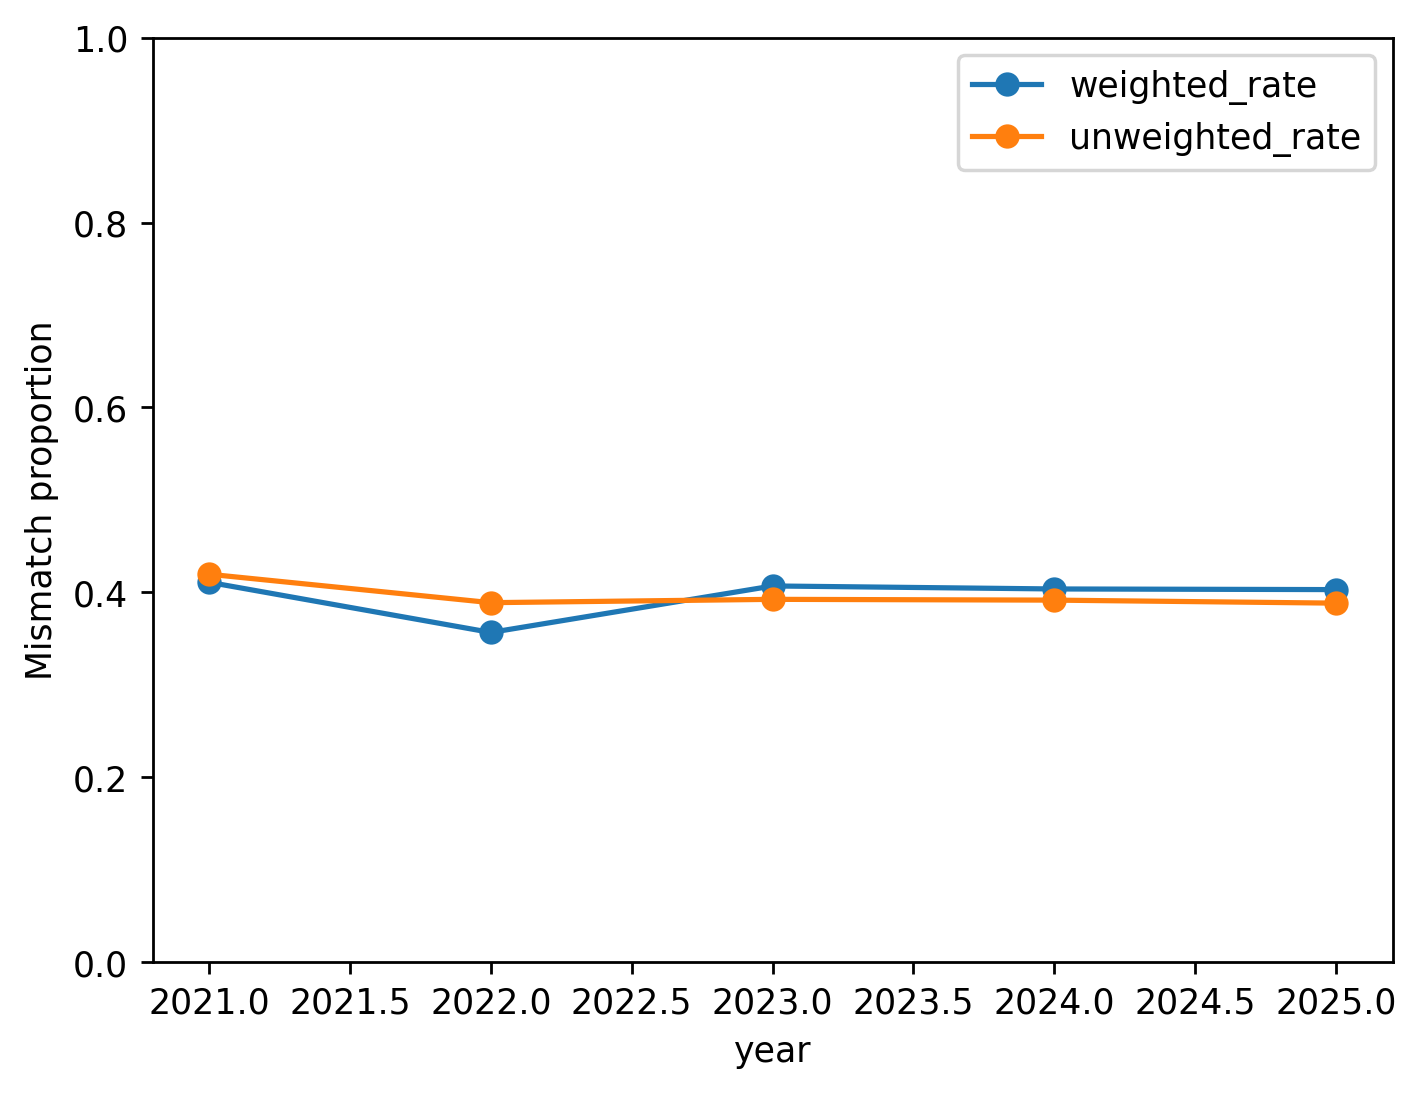
\includegraphics[width=.69\linewidth]{figures/annual_mismatch.png}\caption{Annual weighted and unweighted mismatch among evaluable employed STEM graduates. Source: ENEMDU, project calculations.}\label{fig:annual}\end{figure}

\begin{table}[htbp]\caption{Weighted mismatch by STEM field and sex, 2025. Intervals are approximate 95\% bootstrap intervals.}\label{tab:domains}\centering\small\begin{tabularx}{\linewidth}{Xrrr}\toprule Group & Records & Rate (\%) & Interval (\%)\\\midrule
Natural sciences, mathematics and statistics &442&52.24&43.60--61.42\\
ICT &1082&51.18&41.24--61.28\\
Engineering, industry and construction &3577&34.82&31.11--39.13\\
Men &3769&34.89&31.37--38.64\\
Women &1332&53.67&44.89--61.28\\\bottomrule\end{tabularx}\end{table}
Table~\ref{tab:domains} shows differences by field and sex. Women had a higher weighted mismatch estimate than men in each of the five years. In 2025 the difference was 18.78 percentage points. Age-specific estimates varied, with wide intervals for the youngest and oldest groups. These are descriptive comparisons, not adjusted effects or formal tests of differences.

\subsection{Income and employment conditions}
In 2025 median nominal labour income was USD 898 for compatible records and USD 663 for mismatched records, a difference of USD 235. Adequate employment was more frequent among compatible records, whereas underemployment was more frequent among mismatched records (Table~\ref{tab:income}). The median income ordering was consistent across all five years; mean income was not, as in 2022 the mismatched group had a slightly higher weighted mean. Income was missing or excluded in 72 compatible and 169 mismatched records in 2025, so the income comparison is conditional on retained income responses. Among occupations with at least 50 mismatched records, the leading categories included shop sales assistants (8.34\%) and shopkeepers (6.74\%), weighted shares rather than population counts.
\begin{table}[htbp]\caption{Weighted income and employment conditions in 2025. Income is nominal USD; employment rates use valid activity records.}\label{tab:income}\centering\small\begin{tabular}{lrr}\toprule Indicator & Compatible & Mismatch\\\midrule Records &3121&1980\\ Retained income records &3049&1811\\ Mean income (USD)&1087.65&862.80\\ Median income (USD)&898&663\\ Adequate employment (\%)&82.49&61.36\\ Underemployment (\%)&9.73&18.58\\\bottomrule\end{tabular}\end{table}

\subsection{Predictive performance}
Table~\ref{tab:models} reports weighted 2025 results at the F1 threshold selected in 2024. All fitted classifiers improved AP and ROC-AUC relative to the constant baseline. Logistic regression had the highest ROC-AUC and lowest Brier score; Random Forest had the highest balanced accuracy and specificity, and XGBoost the highest AP and F1. The constant classifier predicts all records as positive at its selected threshold, explaining its high recall and comparable F1. The modest precision and specificity indicate substantial false-positive rates, particularly for logistic regression and XGBoost.
\begin{table}[htbp]\caption{Weighted test performance, 2025, after calibration and validation-based threshold selection.}\label{tab:models}\centering\small\begin{tabular}{lrrrr}\toprule Metric & Constant & LR & RF & XGB\\\midrule ROC-AUC &.5000&.6522&.6434&.6381\\ AP &.4028&.5658&.5579&.5673\\ Precision &.4028&.4142&.4792&.4315\\ Recall &1.0000&.9236&.6974&.8880\\ Specificity &.0000&.1188&.4887&.2108\\ F1 &.5743&.5719&.5681&.5808\\ Balanced accuracy &.5000&.5212&.5931&.5494\\ Brier &.2407&.2233&.2259&.2253\\\bottomrule\end{tabular}\end{table}
\begin{figure}[htbp]\centering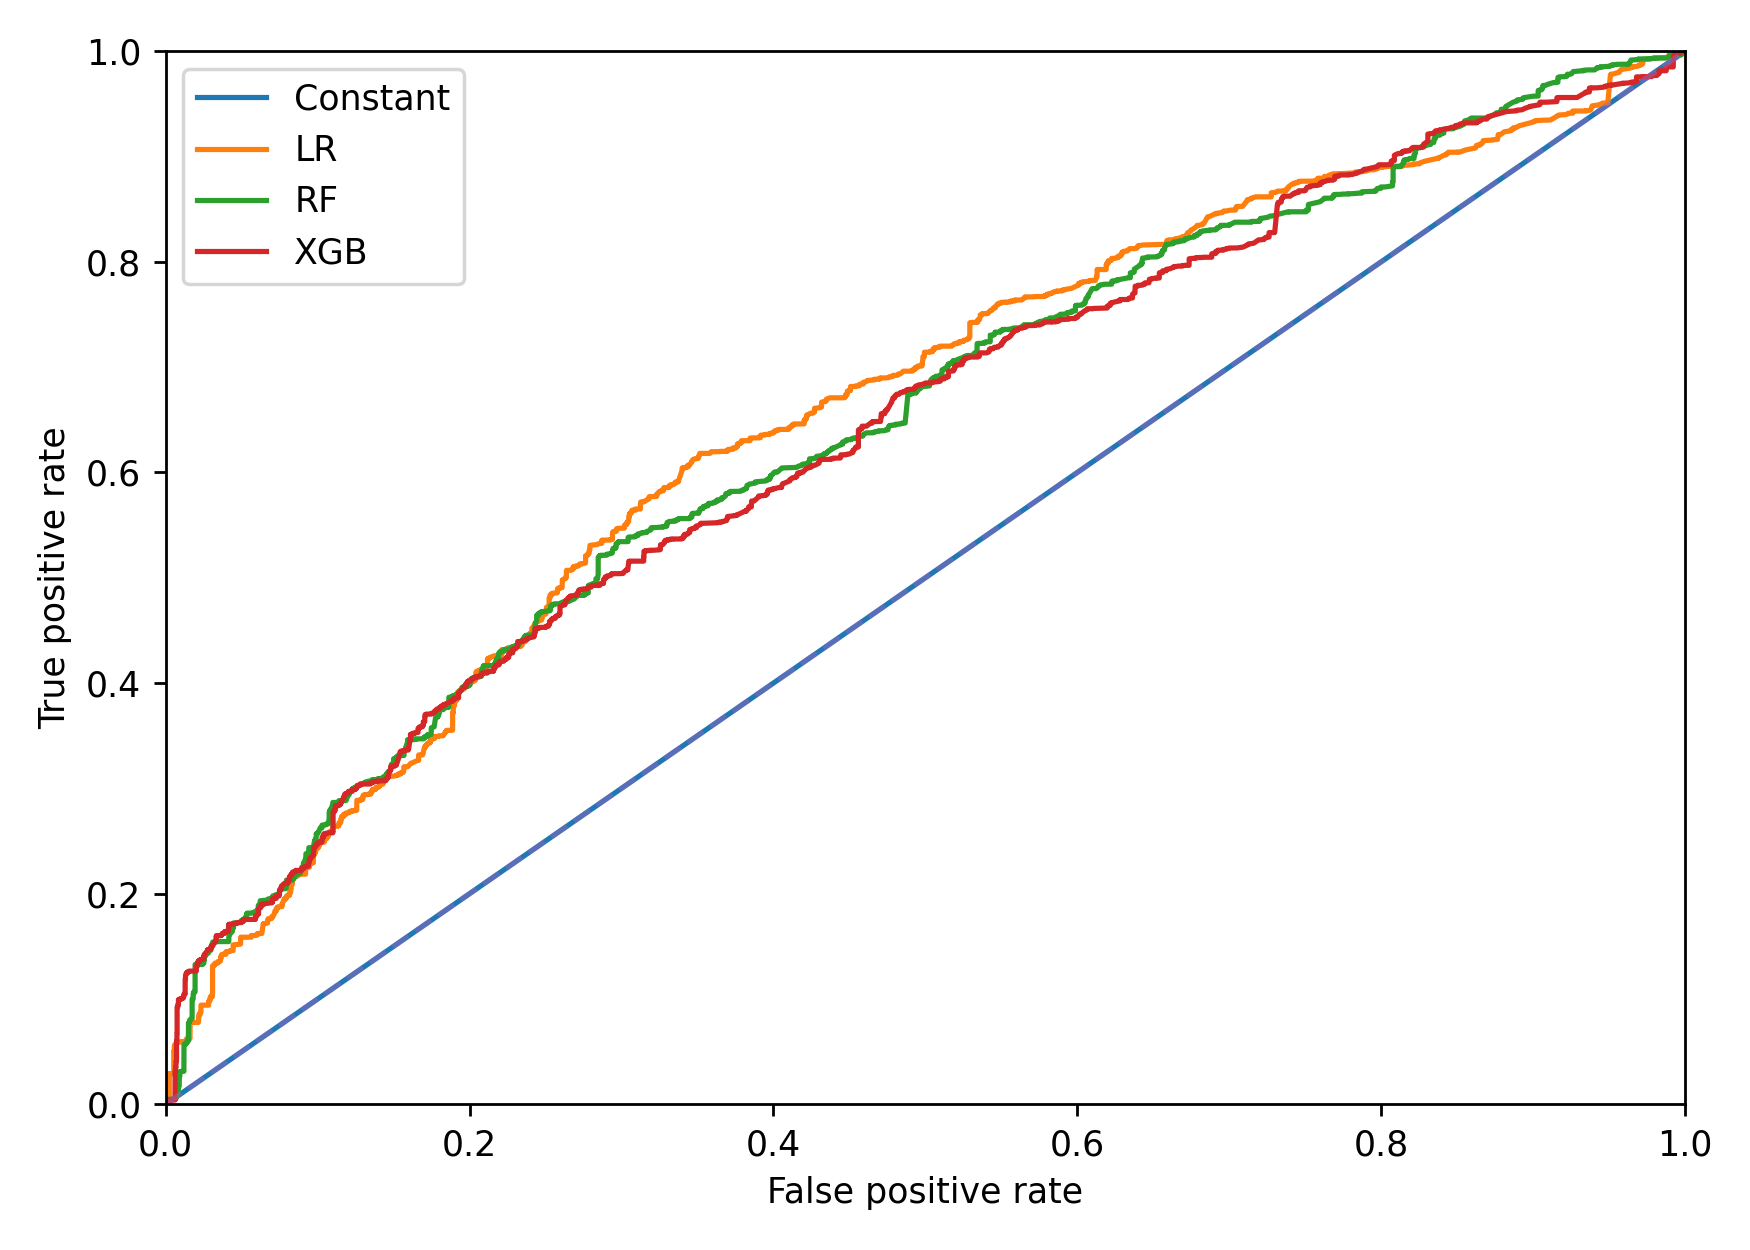
\includegraphics[width=.49\linewidth]{figures/roc.png}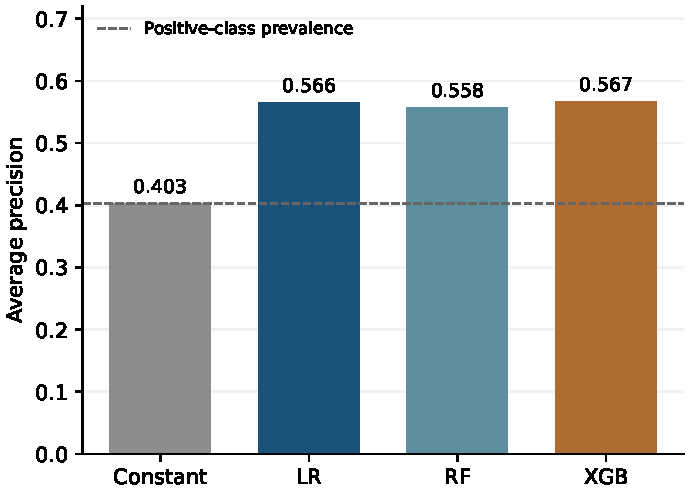
\includegraphics[width=.49\linewidth]{figures/ap_comparison.pdf}\caption{Weighted ROC curves (left) and average precision scores (right) for 2025. The dashed horizontal line denotes positive-class prevalence.}\label{fig:curves}\end{figure}
The paired bootstrap ROC-AUC differences between LR and RF ($-0.0214$ to $0.0373$), LR and XGB ($-0.0136$ to $0.0440$), and RF and XGB ($-0.0176$ to $0.0247$) all included zero. Thus the ordering is descriptive rather than evidence of a clear superiority among fitted models.

\subsection{Interpretation and sensitivity}
Permutation importance identified sex, STEM field and province among the leading predictors in all three models (Figure~\ref{fig:importance}). The leading AP decreases for LR were sex (0.0755), field (0.0365) and province (0.0309); for RF, field (0.0536), sex (0.0411) and province (0.0301); for XGB, field (0.0681), province (0.0481) and sex (0.0417). SHAP was generated for RF but not for XGB due to a software conversion error; the comparable interpretation uses permutation importance.
\begin{figure}[htbp]\centering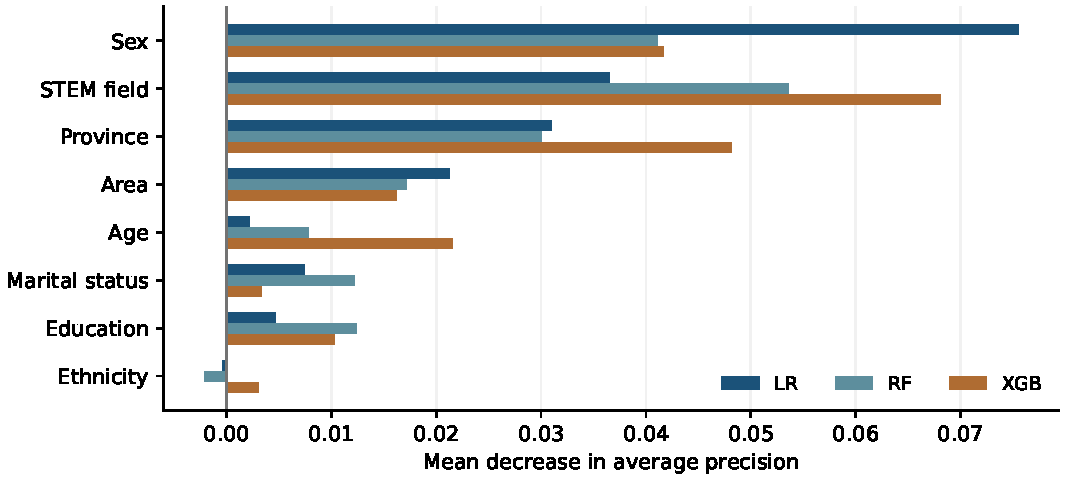
\includegraphics[width=.9\linewidth]{figures/importance_comparison.pdf}\caption{Permutation importance by classifier (mean decrease in AP).}\label{fig:importance}\end{figure}
\begin{table}[htbp]\caption{Weighted ROC-AUC in 2025 under sensitivity scenarios.}\label{tab:sens}\centering\small\begin{tabular}{lrrr}\toprule Scenario & LR & RF & XGB\\\midrule Main &.6522&.6434&.6381\\ Excluding 2021 &.6495&.6383&.6447\\ Without field &.6365&.6151&.6154\\ Unweighted training &.6616&.6476&.6638\\ Candidate household purge &.6502&.6355&.6399\\\bottomrule\end{tabular}\end{table}
Excluding 2021 changed discrimination only modestly. Removing the field reduced ROC-AUC across the three models; unweighted training increased it in the observed test. The candidate household purge reduced training and validation to 12,303 and 3589 records, respectively, while leaving the test unchanged. Performance remained broadly similar (Table~\ref{tab:sens}); this does not establish individual independence. No alternative normative correspondence was evaluated.

\section{Discussion}
The estimated mismatch of approximately four in ten evaluable employed STEM records in 2025 indicates that employment alone does not ensure occupational alignment. This distinction agrees with the conceptual separation of horizontal mismatch, overqualification and skills mismatch discussed by McGuinness et al. and Somers et al. \cite{McGuinness2018,Somers2019}. Robst and Verhaest et al. further distinguish degree-field and qualification-level mismatch; Freeman and Hirsch examine the knowledge content of jobs \cite{Robst2008,Verhaest2017,Freeman2008}. The result is not directly comparable with the OECD figures introduced earlier because the populations, periods and measurement approaches differ. In particular, the rule adapted from Montt \cite{Montt2017} identifies normative compatibility rather than the actual use of skills in a particular job. Task-based or self-reported measurements \cite{Reis2018,Salas-Velasco2021} could classify some records differently.

The differences across STEM fields and sex support the decision to analyse these groups separately. They are consistent with the relevance of heterogeneity discussed in the literature \cite{Kiss2024,Deming2020}, but the observed differences do not identify their mechanisms. Research on STEM career exits and family trajectories, and UNESCO's work on gender barriers in STEM education, offer complementary contexts without establishing the mechanisms in Ecuador \cite{Hunt2016,Cech2019,UNESCO2017}. The income and employment-condition comparisons also provide context for previous studies of mismatch and labour-market outcomes \cite{Montt2017,Takeuchi2023,BotelloPealoza2016,DeLaTorreB2025,Nordin2010}. Bassi et al. provide a wider regional perspective on education and employment \cite{Bassi2012}. The lower median income and lower adequate-employment share of mismatched records should not be interpreted as causal wage penalties. Differences in age, sector, work hours, employment arrangements and missing income could contribute to these patterns.

The predictive comparison answers the research question without assuming that more complex models are better. The highest ROC-AUC was 0.6522, and AP improved over the class prevalence of 0.4028, but the threshold-dependent results show limited individual classification. Logistic regression provides a competitive benchmark, in agreement with the rationale for empirical comparisons in tabular learning \cite{James2023,Grinsztajn2022,McElfresh2023}. The paired intervals do not establish superiority between the fitted classifiers. Sex, field and province were consistently informative; field is partly involved in defining the outcome, so the decrease after excluding it must be understood in light of the label construction. Importance is a measure of predictive contribution rather than an explanation of causality \cite{Molnar2025}.

\subsection{Limitations}
The main limitation is the broad normative correspondence, which combines fields 05 and 06 and uses three-digit occupation groups; it has not been independently validated for Ecuador. A teacher or manager classified as mismatched may still use STEM knowledge. The absence of an alternative documented rule prevents assessing uncertainty in the label itself. Cross-year household identity is not verified, even though the candidate purge provided a conservative sensitivity check. The 2025 data were inspected during the first analysis and the corrected AP evaluation is not a wholly new holdout. Bootstrap intervals are approximate under the survey design and singleton strata; they do not account for label uncertainty. Income comparisons exclude missing/non-finite values and the nonresponse sentinel 999999, but retain recorded negative incomes (22 in 2025); the interpretation of these values requires confirmation. Nominal values are not adjusted for inflation. The 2021 precision issue also limits exact-degree analysis. Finally, the analysis concerns employed and evaluable graduates only: it cannot measure vacancies, shortages, unemployment risk, or future career trajectories; the OECD distinguishes mismatch from skills shortages and surpluses \cite{OECD2017}. Further research could validate the correspondence with occupational experts or task-level information and assess model performance on a genuinely new annual sample.

\section{Conclusions}
This study constructed a reproducible normative indicator of field-of-study mismatch among employed STEM university graduates using annual ENEMDU data from 2021--2025. Of the 24,525 evaluable person-period records, the weighted mismatch estimate for 2025 was 40.28\%. Differences by field and sex, together with lower median nominal income and less favourable employment conditions in the mismatched group, demonstrate the value of examining occupational compatibility alongside general employment indicators.

The machine learning models showed modest predictive performance. Logistic regression achieved the highest ROC-AUC, XGBoost the highest AP and Random Forest the highest balanced accuracy; no clear overall winner was established. Sex, STEM field and province contributed consistently to prediction. The sensitivity analyses support the stability of several findings under changes in training specification, but do not resolve the limitations of the normative label or longitudinal linkage. These findings provide a basis for further investigation of educational and occupational alignment rather than for individual employment decisions or causal policy recommendations.

\funding{No external funding was reported for this academic project.}
\dataavailability{The analysis uses public ENEMDU annual microdata and INEC classifications. The computational workflow and replication materials are available at \url{https://github.com/Steven735-star/Ecuador-STEM-Mismatch-2021-2025}.}
\reftitle{References}
\bibliography{references}
\end{document}
